\section{Data Sources} \label{data_sources}

\subsection{Mobile Phone Data Source}

The data used in this study consist of a set \( \mathP \) of \textit{Call Detail Records} (CDRs), composed of voice calls and text messages from a Mexican telecommunication company (\textit{telco}) for a 3 month long period.

Every CDR \( p \in \mathP \)  contains the anonymized phone numbers of the caller and callee \( \left< p_o, p_d \right> \), the start time \( p_t \), and, in the case of voice calls, the call duration \( p_s \). The latitude and longitude of the antennae used for the calls \( \left< p_y, p_x \right> \), are also given for a small subset of the data.

Given that our collection \( \mathP \) of CDRs are coming from the same telephone company, we are able to reconstruct all communication links between clients of this company, as well as communications between the clients and other users, but we have no information on communications where neither users are clients of our telco company.

If we define \( N \) as the users of the telco, and \( \mathP_N \subseteq \mathP \) as the calls where \( \left( \forall p \in \mathP_N \right) p_o \in N \wedge p_d \in N \), we can create a communications graph \( \mathG \) which contains only the users from the telco and all of the calls between them.

%With the data provided to us by the telco, \( \mathG \) contains \num{72107108} users who made \num{72107108} calls and sent \num{634225740} text messages in this period of 3 months.

\subsection{Banking Information}

For this study we also used account balances for over 10 million clients of a bank in Mexico for a period of 6 months, denoted \( \mathB \). The data for each client \( b \in \mathB \) contains his phone number \( b_p \), anonymized with the same hash function used in \( \mathP \), and the reported income of this person over 6 months \( b_{s_0}, \ldots, b_{s_5} \). We average these 6 values to get \( b_s \), an estimate of a user's income.

The bank also provided us with demographic information for a set of users \( \mathA \subseteq \mathB \). For each user \( u \in \mathA \) we are given  the age \( u_a \) and the gender \( u_g \) of the user. This allowed us to observe differences in the income distribution according to the age and gender. In another line of work, homophily respect to the age has been observed in \cite{brea2014} and used to generate inferences.

\begin{figure}[h]
\begin{center}
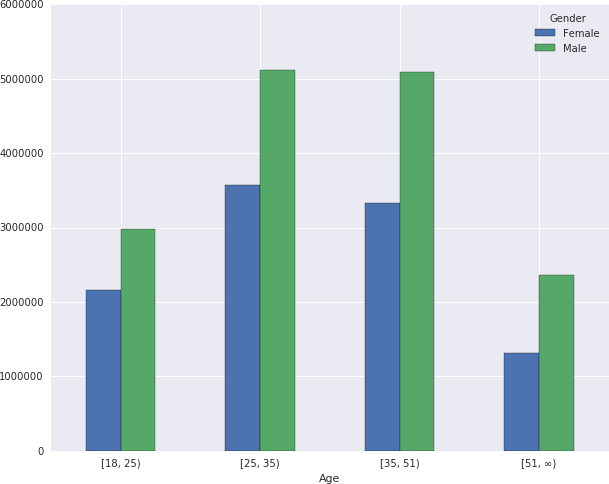
\includegraphics[width=0.8\columnwidth]{figures/gender_age_bar3/gender_age_bar3.png}
\caption{ \protectReplace this text with your caption}
\label{gender_age_bar}
\end{center}
\end{figure}

\begin{figure}[h]
\begin{center}
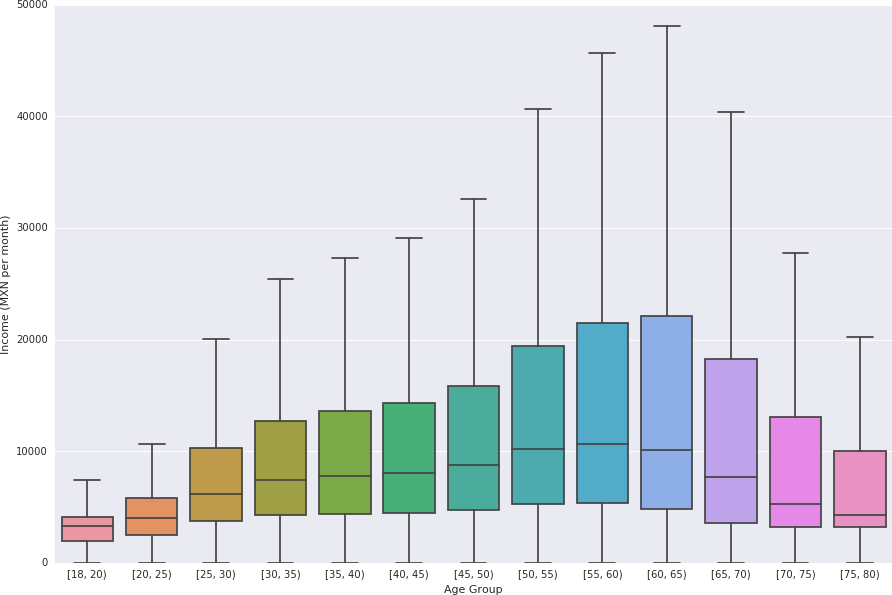
\includegraphics[width=0.95\columnwidth]{figures/income_age_boxplot4/income_age_boxplot4.png}
\caption{ \protectReplace this text with your caption}
\label{income_age_boxplot}
\end{center}
\end{figure}

Figure~\ref{gender_age_bar} shows the distribution of users in $\mathB$, according to
their age range and gender.
Figure~\ref{income_age_boxplot} shows the distribution of income, according to the age range (generated by taking 5 years intervals for the age).
It is interesting to note how the median income increases with the age, up to 65 years old (the retirement age in Mexico). After 65 years old, the median income rapidly decreases.


\subsection{Bank and Telco Matching}

Since the phone numbers in each call of the telco data $ p_o $ and $ p_d $ are anonymized with the same hash function as the phone number in the bank data, $ b_p $, we can match users to his unique phone create another social graph: 
$$ G = \mathP \bowtie_{_{p_o = b_p}} \mathB \bowtie_{_{p_d = b_p}} \mathB $$ 
where $\bowtie$ denotes the inner join operator.
$G$ includes income information for the subset of the social graph that appears in the bank data.
This graph has a total of \num{2027554} nodes with \num{5044976} edges, which represent \num{29599762} calls. % and \num{5476783}.

\subsection{Outlier Filtering}

The dataset contains information about bank and telco users, some of which may not directly correspond to a human user who exclusively users the telco and the bank used in this study, or may have no useful information for our research. Most of the telco users in the first case are already filtered by the intersection (\textsc{inner join}). To make sure the users are relevant enough to this work, we only use the users which have:

\begin{itemize}
	\item More than 5 calls in either direction.
	\item A monthly income of at least \$\num{1000}.
	The value is expressed in Mexican pesos (MXN)\footnote{At the time of writing (May 22, 2016), 1000 Mexican pesos are equivalent to 54 US dollars.}.
	\item A monthly income in the \num{99}th percentile
	(i.e. we filter users with a monthly income in the top 1\%).
\end{itemize}
